\documentclass[a4paper,12pt]{article} 

% packages and main settings
\usepackage[left=3cm, right=2cm, top=2cm, bottom=2cm]{geometry}
\usepackage[english]{babel}    
\usepackage[utf8]{inputenc}  
\usepackage[T1]{fontenc}        
\usepackage{lmodern}            
\usepackage{microtype}          
\usepackage{amsmath}
\usepackage{amsfonts, amsthm, amssymb, graphicx, booktabs}
\usepackage{bm} %bold epsilon
\usepackage{newclude}   
\usepackage{placeins}  %surpresses floating tables
\usepackage[labelfont=bf]{caption} %Figure etc steht dann in small caps 
\usepackage[labelsep=period]{caption} % dot after figure, table caption.
\usepackage[flushleft]{threeparttable} % for notes below table
\usepackage{multirow} % for table cell merge along rows
\usepackage{graphicx} % to adjust tablesize to textwidth
\usepackage{caption}  % for centered captions
\usepackage{float} % to set of autopositioning of tables
\usepackage[bottom,hang,flushmargin]{footmisc} % forces footnotes to the bottom
\usepackage{setspace}           % Fuer 1.5 fachen Zeilenabstand  
\onehalfspacing % 1.5 cm Zeilenabstand
%Bibtex
\usepackage[round,sort&compress]{natbib}

\bibliographystyle{chicago} % chicago bib style like in AER
\usepackage[hidelinks]{hyperref} % fuer links und verweise. Cleverref ist eigentlich besser. 


% Create header. The header must be surpressed for 
% every first page per section and a solution
% for the Appendix is used in the respective subfile.
\usepackage{fancyhdr}
\pagestyle{fancy}
\fancyhf{}
\chead{\nouppercase{\textit{\leftmark}}}
\cfoot{\thepage}
\renewcommand{\headrulewidth}{0pt} % no vertical line

%\usepackage{lipsum}  % check if formats work

\usepackage{afterpage} %clearpage w/o pagebreak for "header bug"

% Expectation symbol
\DeclareMathOperator*{\E}{\mathbb{E}}

% thin space, limits underneath in displays
% for strike through
\DeclareMathOperator*{\argmax}{argmax}
\newcommand*{\defeq}{\stackrel{\text{def}}{=}}
\usepackage[normalem]{ulem}
% try to use strikeout in section headers and others
\DeclareRobustCommand{\hsout}[1]{\texorpdfstring{\sout{#1}}{#1}}

% for gray table row color
\usepackage[table]{xcolor}

% decimal dot alignment in table columns
\usepackage{siunitx}

% for footnotes in table
\usepackage[flushleft]{threeparttable}

% for underbar
\newcommand{\ubar}[1]{\text{\b{$#1$}}}

\usepackage{tikz}

% Setup for urls
\usepackage{url}

\defcitealias{Respy-Stenzel.2019}{\textit{respy}}
\defcitealias{Gabler.2019}{\textit{estimagic}}
\defcitealias{Stenzel.2020}{\textit{Master's Thesis Replication Repository}}
\defcitealias{NLSY79}{NLSY79}


\usepackage{tikz}
\begin{document}

\newpage % delete after section is complete

\section{Model and Estimation}
\thispagestyle{plain} % suppress header on first page
This section introduces the model whose uncertainty is quantified and emphasizes the main economic, mathematical and computational aspects. It is the partial equilibrium, dynamic model of occupational choice developed in \cite{Keane.1994} (henceforth KW94). In their survey of dynamic discrete choice structural models, \cite{Aguirregabiria.2010} assign this model to the more general class of Eckstein-Keane-Wolpin models. I largely follow their notation to ease comparisons with other models and, most importantly, to ease the explanation of the estimation method. Eckstein-Keane-Wolpin models are used to explain educational and occupational choices at the individual level. \\
\newline
The class of Eckstein-Keane-Wolpin models is structural. This means that, from the perspective of an econometrician, the model structure allows for the estimation of relationships between observable and unobservable variables. This requires the model to be solved for the agents' policy. The policy is the set of rules which describe the agents' optimal behaviour. The relationships between observables and unobservables are governed by exogenous parameters. These parameters may, for example, be utility parameters or distributional parameters which describe the processes of unobserved shocks. Therefore, the exogenous parameters can be estimated given a dataset of observable endogenous variables. Besides the observable states, the observable endogenous variables may also comprise of other parameters like, for instance, payoffs. Estimates for the exogenous parameters allow to use simulations (of states) in order to analyse counterfactual policy scenarios. These policies are represented by changes in some exogenous parameters. For instance, \cite{Keane.1997} obtain the following two results based on data from the \citetalias{NLSY79}: First, unobserved heterogeneity in the endowment at age sixteen accounts for almost 90\% of the variance in lifetime utility whereas shocks to productivity explain 10\%. Second, a college tuition subsidy of 2,000 USD increases high school and college graduation by 3.5\% and 8.4\%, respectively.\\
\newline
As the research code for \cite{Keane.1997} is currently in alpha-version, this thesis studies the predecessor model in KW94. The main differences are that the model in KW94 does not contain unobserved permanent agent heterogeneity in endowment and that its choice-specific utility functions feature fewer covariates. This difference in complexity implies a decrease of the computational burden for the UQ but also a substantially worse fit to the data. In fact, this thesis does not use estimates from real data but estimates from simulated data based on arbitrary parameters from KW94.\\
\newline
The section proceeds as follows: First, I introduce the  KW94 model specification embedded in the more general Eckstein-Keane-Wolpin framework. This embedding provides additional context to the reader. In the next step, the estimation method simulated maximum likelihood is presented. This approach is used for the structural estimation of the exogenous model parameters. After remarks on the numerical implementation, I show the estimation results. They include the estimates, the standard errors, and the correlations for all parameters. These results constitute the mean vector and the covariance matrix, which are used to characterize the joint input distribution for the UQ in the next section. The section ends by describing the QoI choice.

\subsection{\cite{Keane.1994}}

\cite{Aguirregabiria.2010} define Eckstein-Keane-Wolpin models by four characteristics. The first characteristic is that these models allow for permanent unobserved heterogeneity between agents. The simpler model by KW94 considered here does not use this option in contrast to \cite{Keane.1997}. The other three characteristics are as follows:
\begin{enumerate}
	\item Unobservable shocks $\varepsilon_t$ do not have to be additively separable from the remainder of the utility functions.
	\item Shocks $\varepsilon_t$ can be correlated across choices $a_t$.
	\item Observable payoffs, or wages, $W_{a,t}^{-}$ are not conditionally independent from the unobservable shocks $\varepsilon_t$ given the observable choices $a_t$ and the observable part of the state vector $\bold{s_t^-}$. The reason is that wage shocks enter the wage function directly. If the agent decides against choices with observable payoffs that depend on $\varepsilon_t$, these payoffs can not be observed. Therefore, positive shocks and the observation of payoffs for the same choice are positively correlated.
\end{enumerate}

\noindent
This paragraph describes the Eckstein-Keane-Wolpin model framework without permanent agent heterogeneity in the context of occupational choices as in KW94. In this setting, agents only differ in their draws of unobserved shocks $\varepsilon_t$.

In each period, a representative agent receives utility $U$. This utility depends on the state space and on choice $a$ in period $t \in \{0,1,2,...,T\}$. Choices are mutually exclusive. The state space is the set of information in each period which is relevant for present and future utilities. It is split into an observable part $\bm{s_t^-}$ and an unobservable part $\pmb{\varepsilon_{t}}$. Choice $a_t$ itself is also a function of the state space. This function is the decision rule, or policy, under which the rational agent chooses his utility for period t. For convenience, or to view utility and choices from different angles, $U$ is denoted as function of only the states, as a function of $a_t$ and the states, or as a function of function $a_t(\bold{s_t^-}, \pmb{\varepsilon_t})$ and the states.

For some occupation alternatives, utility and prior decisions may be intertemporally connected: Agents receive a higher utility if they accumulated skills in past occupations that are useful for these alternatives. Other occupations may not reward experience. The observable part of the state space comprises the period, the work experience and the choice in the previous period. The unobservable part of the state space consists of the alternative-specific shocks $\{\varepsilon_{a,t}\}_{a \in A}$. Figure \ref{fig:order} depicts the series of events.





\begin{figure}[H]
	\caption{Series of events} \label{fig:order}
	\vspace{-0.0cm}
	
	\begin{center}        
		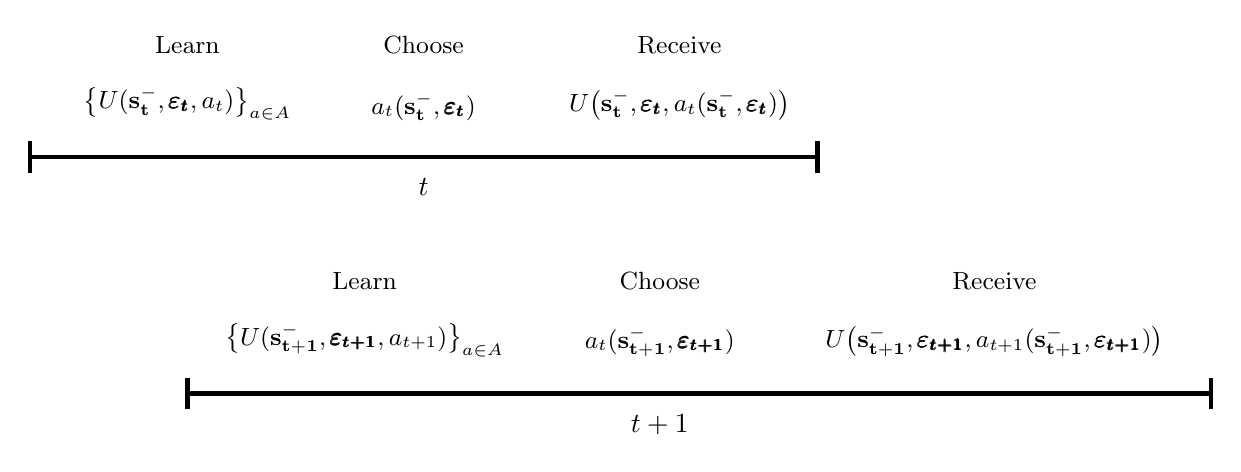
\begin{tikzpicture}
		% upper part
		\draw [ultra thick] (0,0) -- (10,0);
		\foreach \x in {0,10}
		\draw [ultra thick] (\x cm,0.2) -- (\x cm, -0.2);
		\small % derease fontsize
		\draw (2.0,0) node[above=0.35cm] {$\big\{U(\bold{s_t^-}, \pmb{\varepsilon_t},a_t)\big\}_{a \in A}$};
		\draw (5.0,0) node[above=0.35cm] {$a_t(\bold{s_t^-}, \pmb{\varepsilon_t})$};
		\draw (8.25,0) node[above=0.35cm] {$U\big(\bold{s_t^-}, \pmb{\varepsilon_t},a_t(\bold{s_t^-}, \pmb{\varepsilon_t})\big)$};
		
		\draw (2.0,0) node[above=1.2cm] {Learn};
		\draw (5.0,0) node[above=1.2cm] {Choose};
		\draw (8.25,0) node[above=1.2cm] {Receive};
		
		\normalsize %reincrease fontsize
		\draw (5.0,0) node[below=0.15cm] {$t$};
		
		%lower part
		\draw [ultra thick] (2.0,-3) -- (15,-3);
		\foreach \x in {2.0,15}
		\draw [ultra thick] (\x cm,-2.8) -- (\x cm, -3.2);
		\small % derease fontsize
		\draw (4.25,-3) node[above=0.35cm] {$\big\{U(\bold{s_{t+1}^-}, \pmb{\varepsilon_{t+1}},a_{t+1})\big\}_{a \in A}$};
		\draw (8.0,-3) node[above=0.35cm] {$a_t(\bold{s_{t+1}^-}, \pmb{\varepsilon_{t+1}})$};
		\draw (12.25,-3) node[above=0.35cm] {$U\big(\bold{s_{t+1}^-}, \pmb{\varepsilon_{t+1}},a_{t+1}(\bold{s_{t+1}^-}, \pmb{\varepsilon_{t+1}})\big)$};
		
		\draw (4.25,-3) node[above=1.2cm] {Learn};
		\draw (8.0,-3) node[above=1.2cm] {Choose};
		\draw (12.25,-3) node[above=1.2cm] {Receive};
		
		\normalsize %reincrease fontsize
		\draw (8.0,-3) node[below=0.15cm] {$t+1$};      
		
		%\draw (2.35,0) node[above=6pt, align=center] {(estimation \\ window]};
		\end{tikzpicture}
	\end{center}
\end{figure}

\noindent
At the beginning of each period $t$, the agent recognizes the reward shocks $\{\varepsilon_{a,t}\}_{a \in A}$ (as opposed to the observer), and the shocks become part of the unobserved state space $\pmb{\varepsilon_t}$. Thus, the alternative-specific utilities $\{U(\bold{s_t^-}, \pmb{\varepsilon_t},a_t)\}_{a \in A}$ are known to the agent in period $t$. However, he can only form expectations about rewards in the future as the alternative-specific shocks $\{\varepsilon_{a,t}\}_{a \in A}$ are stochastic. The specification in KW94 assumes the rewards shocks $\{\varepsilon_{a,t}\}_{a \in A}$ to be serially uncorrelated. Therefore, prior shocks do not enter the state space. Next, the agent chooses his occupation $a_t$ based on the state space information and according to his policy rule $a_t(\bold{s_t^-}, \pmb{\varepsilon_t})$. Then he receives the occupation-specific reward. The reward can be written as a function composition of utility and policy. This flow repeats for each $t < T$. The computation of the optimal policy is sketched in the next paragraph.\\
\newline
Agents are rational and forward-looking. Future utilities are subject to time discount factor $\delta  \in [0,1]$. Hence, they choose their optimal sequence of occupations by maximizing the remaining expected, discounted life-time utility. This maximal value is given by value function $V(\bold{s_t^-}, \pmb{\varepsilon_t})$ in (\ref{eq:value-function}). Like utility $U$, I also write value function $V$ with different emphasis on occupation choice $a_t$.
\begin{align} \label{eq:value-function}
V(\bold{s_t^-}, \pmb{\varepsilon_t}) = \max_{\{a\}_{t=0}^T} \bigg\{ \sum_{t=0}^T \delta^t \int_{\pmb{\varepsilon_t}} U(\bold{s_{t}^{-}},\pmb{\varepsilon_{t}}, a_{t}) f(\pmb{\varepsilon_{t}})d^{|A|}\pmb{\varepsilon_{t}}\bigg\}
\end{align}
Value $V$ depends directly on time $t$ because $T$ is finite. Together with the discount factor $\delta$, this typically induces life-cycle behaviour. For example, agents invest more in the earlier time periods and work (and consume) more in the following periods. As $\{\varepsilon_{a,t}\}_{a \in A}$ are the only random parameters and serially independent, the expectation of $U(\bm{s_{t}^{-}},\pmb{\varepsilon_{t}}, a_{t})$ is given by the $|A|$-dimensional integral of U multiplied by the joint probability density function $f(\pmb{\varepsilon_{t}})$ with respect to $\pmb{\varepsilon_{t}}$. $|A|$ denotes the number of occupation choices.

Coursely sketched, the approach to solve the above maximization problem is given by the dynamic programming problem characterized by the Bellman equation (\cite{Bellman.1957})\footnote{For more details, see \cite{Raabe.2019}, p. 9-19.} that breaks up the problem in (\ref{eq:value-function}) into more tractable sub-problems along the time dimension.
\begin{align} \label{eq:Bellman}
V(\bold{s_t^-}, \pmb{\varepsilon_t}) = \max_{a_t} \bigg\{ U(\bold{s_t^-}, \pmb{\varepsilon_t}, a_t) + \delta \int_{\pmb{\varepsilon_t}} \max_{a_{t+1}} V(\bold{s_{t+1}^{-}},\pmb{\varepsilon_{t+1}},a_{t+1}) f(\pmb{\varepsilon_{t+1}})d^{|A|}\pmb{\varepsilon_{t+1}}\bigg\}
\end{align}
\noindent
The Bellman equation shows, that solving for the whole sequence of policy functions ${\{a\}_{t=0}^T}$ is equivalent to solving iteratively for each optimal, period-specific policy function $a_t(\bold{s_t^-}, \pmb{\varepsilon_t})$. For this purpose, choose $a_t$ for each period such that the current period utility and the discounted expected future lifetime utility (given the optimal choice of $a_{t+1}$) are maximized. The finite time horizon eases the problem as the value function for the last period $T$ simplifies to $V(\bold{s_T^-}, \pmb{\varepsilon_T}) = \max_{a_T} U(\bold{s_T^-}, \pmb{\varepsilon_T}, a_T)$.\footnote{More precisely, a finite time horizon in contrast to an infinite time horizon implies that the solution does not require, first, to  guess the future value function for an arbitrary last time period, and, second, to iterate backwards in time to obtain a converged value function. On the other hand, the finitite time horizon complicates the solution, because it requires one policy function for each time period vice versa solely one policy function for the converged value function of the infinite horizon problem.} With this condition, the problem can be solved for all states by iterating backwards: First, one solves for the final period policy $a_T(\bold{s_T^-}, \pmb{\varepsilon_T})$. Then this sub-result is plugged in the future value function on the right hand sight of (\ref{eq:Bellman}) to solve for $a_{T-1}(\bold{s_{T-1}^-}, \pmb{\varepsilon_{T-1}})$, and so forth until $t=1$. By emphasizing time as a dimension, the policies can also be summarized as one function $a(\bold{s_t^-}, \pmb{\varepsilon_t})$. Given random draws for the  unobservable shocks $\pmb{\varepsilon_t}$ for each period, this policy is used to simulate the occupational paths for a number of agents.\\

\noindent
This paragraph addresses the alternative-specific utility functions $\{U(\bold{s_t^-}, \pmb{\varepsilon_t},a_t)\}_{a \in A}$ that finally pin down the model in KW94.

There are four different occupations, $b$, $w$, $e$ and $h$, of which occupations $b$ and $w$ are defined by the same type of utility function. In the following, I will roughly explain how the first two utility functions model characteristics for working in the blue- and in the white-collar sector and how the latter two equations sketch receiving institutional education and staying at home. The parametrization that distinguishes the blue from the white-collar sector and additional intuition is given later in subsection Estimation Results and in Table \ref{tab:params}.

It is assumed that there is a direct mapping from USD to utility. Based on this, the utility functions for occupation $b$ and $w$, $U_b$ and $U_w$, equal the occupation-specific wage, $W_{b,t}$ and $W_{w,t}$, in USD. The wage equations are given by the Mincer equation for earnings (\cite{Mincer.1958}):
\begin{equation} \label{eq:returns_b_w}
\begin{aligned}
U(\bold{s_t^-}, \pmb{\varepsilon_t},b) &= W_{b,t}^{-} = \text{exp}\big\{\beta^b + \beta_e^b x_{e,t} + \beta_b^b x_{b,t} + \beta_{bb}^b x^2_{b,t} + \beta_w^b x_{w,t} + \beta_{ww}^{b} x^2_{w,t} + \varepsilon_{b,t}\big\} \\
U(\bold{s_t^-},\pmb{\varepsilon_t},w) &= W_{w,t}^{-} = \text{exp}\big\{\beta^w + \beta_e^w x_{e,t} + \beta_w^w x_{w,t} + \beta_{ww}^w x^2_{w,t} + \beta_b^w x_{b,t} + \beta_{bb}^{w} x^2_{b,t} + \varepsilon_{w,t}\big\}
\end{aligned}
\end{equation}
\newline
Both equations comprise of a constant term, years of schooling $x_{e,t}$, linear and quadratic terms of occupation experience, and cross-occupational experience and the  respective shocks in $\pmb{\varepsilon_{t}}$. $\pmb{\beta}$ is the vector of coefficients that multiply the previously defined terms.\footnote{The notation for $\pmb{\beta}$ includes two references. The superscript indicates the occupation-specific utility that contains the coefficients. The subscript indicates the occupation-specific experience or abbreviates the condition that regulates the coefficients. Thus, coefficients for constant terms do not have a subscript. Twice the respective subscript mark coefficients for quadratic terms.} These coefficients are called covariates by many structural economists.

The utilities for education, or schooling, and staying at home are given by the functions in (\ref{eq:returns_e_h}). These functions are also called non-pecuniary rewards.
\begin{equation} \label{eq:returns_e_h}
\begin{aligned}
U(\bold{s_t^-}, \pmb{\varepsilon_t},e) &= \beta^e + \beta_{he}^e \bold 1(x_{e,t} \geq 12) + \beta_{re}^e(1-\bold1(a_{t-1}=e)) + \varepsilon_{e,t} \\
U(\bold{s_t^-},\pmb{\varepsilon_t},h) &= \beta^h + \varepsilon_{h,t} \\
\end{aligned}
\end{equation}
\noindent
$\beta^e$ is the consumption reward of schooling. Function $\bold 1(x_{e,t} \geq 12)$ indicates whether an agent has completed high school. $\beta_{he}^e$ is the tuition fee on higher or post-secondary education and $\beta_{re}^e$ is an adjustment cost for returning to school when the agent chose another occupation the previous period ($a_{t-1}\neq e$). $\beta^h$ is the mean reward for staying at home.

Write $\{\varepsilon_{a,t}\}_{a \in A}$ as vector $\pmb{\varepsilon_{a,t}}$. It is assumed that $\pmb{\varepsilon_{a,t}}$ follows a joint normal distribution, such that $\pmb{\varepsilon_{a,t}} \sim \mathcal{N}(0,\,\pmb{\Sigma_\varepsilon})$. \pmb{$\Sigma_\varepsilon$} denotes the covariance matrix for shocks $\pmb{\varepsilon_{a,t}}$. $\sigma_a^{2}$ and $\sigma^{2}_{a(j),a(k\neq j)}$ denote the alternative-specific variances and covariances in \pmb{$\Sigma_\varepsilon$}. Shocks are serially uncorrelated. Indices $\{j,k\} \in \mathbb{N}$ are used to denote subsets of $a$.

Finally, there is a bijective mapping from periods $t$ to age $16$ to $65$. The next subsection describes the estimation method.

\subsection{Simulated Maximum Likelihood Estimation}

To estimate the exogenous model parameters, the approach that this thesis and also KW94 use is the simulated maximum likelihood method (\cite{Albright.1977})\footnote{See \cite{Aguirregabiria.2010}, p. 42-44 and \cite{Raabe.2019}, p. 21-26 for more details.}.

This method can be applied to a set of longitudinal data on occupational choices $a_t$ and, if available, wages $W_{a,t}^{-}$ of a sample of $i \in I$ individuals starting from age 16. To distinguish from its functional form, let $\mathcal{W}^{-}_{a(k),t}$ henceforth denote the measured wages. For each period $t$, the recorded choices $a_0$, ..., $a_{t-1}$  imply the occupation-specific experiences $x_{a,t}$. Together with $t$, they constitute the observable state vector $\bold{s_t^-}$. Consequently, the measured, observable endogenous variables are $\pmb{\mathcal{D}}\defeq(\bold{s_t^-},\mathcal{W}^{-}_{a,t})$. Given this setup, the goal is to estimate the exogenous model parameters $\pmb{\theta}\defeq(\delta, \pmb{\beta}, \pmb{\Sigma_\varepsilon})$.\footnote{Improvements in this thesis' estimation over KW94 are that, first, it is not assumed that the standard errors of the parameters estimates are uncorrelated, and, second, that $\beta$ is not left out of the estimation.} Thus, in the following, every probability is a function of the exogenous model parameters $\pmb{\theta}$.
The approach to compute the likelihood function $L_{\pmb{\mathcal{D}}}(\pmb{\theta})$ of the observables in the data begins with the individual latent variable representation in period $t$.
\begin{align}
a_t = \argmax_a V(\bold{s_t^-},\pmb{\varepsilon_t},a_t)
\end{align}
As $a_t$ and $\bold{s_t^-}$ are known, the next step is to derive the unobservable shocks $\pmb{\varepsilon_t}$ in terms of $a_t$ and $\bold{s_t^-}$. Therefore, write the set of shocks for which the alternative-specific value function $V(\bold{s_t^-},\pmb{\varepsilon_t},a_t(j))$ is higher than the other value functions $V(\bold{s_t^-},\pmb{\varepsilon_t},a_t(k\neq j))$ as
\begin{align}
\pmb{\varepsilon_t}(a_t(j),\bold{s_t^-}) \defeq \{\pmb{\varepsilon_t}|V(\bold{s_t^-},\pmb{\varepsilon_t},a_t(j)) = \max_{a_t} V(\bold{s_t^-},\pmb{\varepsilon_t},a_t)\}).
\end{align}
Note that the set condition is a function of the unobservable model parameters $\pmb{\theta}$.

Consider first the case of non-working alternatives $a_t(j) \in [e,h]$. The probability of choosing $a_t(j)$ is the probability of set $\pmb{\varepsilon_t}(a_t(j),\bold{s_t^-})$. This probability equals the integral of the probability distribution function $f(\pmb{\varepsilon_t})$ over all elements of set $\pmb{\varepsilon_t}(a_t(j),\bold{s_t^-})$ with respect to $\pmb{\varepsilon_t}$. Formally,
\begin{align}
\text{p}\big(a_t(j) | \bold{s_t^-}\big) = \int_{\pmb{\varepsilon_t}(a_t(j),\bold{s_t^-})} f(\pmb{\varepsilon_t}) d^{|A|} \pmb{\varepsilon_t}.
\end{align}
\noindent
The second case is $a_t(k) \in [b,w]$. Assuming the dataset contains wages for the working alternatives $a_t(k)$, the probabilities of choosing $a_t(k)$ take a few steps more to compute. First, note from the wage equations that the the alternative-specific shocks $\pmb{\varepsilon_{a,t}}$ are log normally distributed. Second, in contrary to the non-working alternatives, using (\ref{eq:returns_b_w}), the shocks can directly be expressed as a function of the alternative-specific model parameters $\pmb{\beta_{a(k)}}$ by inserting the inferred alternative-specific experiences $\pmb{x_{a(k),t}}$ into $W_{a(k),t}$ and subtracting the expression from the observed wage $\mathcal{W}^{-}_{a(k),t}$ for each individual. Both wages are logarithmized. Thus,
\begin{align} \label{eq:epsilon}
\varepsilon_{a(k),t} = \text{ln}(\mathcal{W}^{-}_{a(k),t}) - \text{ln}(W_{a(k),t}^{-}).
\end{align}
Third, the alternative-specific shocks $\pmb{\varepsilon_{a,t}}$ are not distributed independently. Since $\varepsilon_{a(k),t}$ can be inferred from the
observed wage $\mathcal{W}^{-}_{a(k),t}$, this information can be used to form the expectation about the whole error distribution. Therefore, using the conditional probability density function $f(\pmb{\varepsilon_t}|\varepsilon_{a(k),t})$, the probability of choosing occupation $a_t(k)$ conditional on observed states and wages writes

\noindent
\begin{align} \label{eq:prob-choice}
\text{p}\big(a_t(k) | \bold{s_t^-},W^{-}_{a(k),t}\big) = \int_{\pmb{\varepsilon_t}(a_t(k),\bold{s_t^-})} f(\pmb{\varepsilon_t}|\varepsilon_{a(k),t}) d^{|A|} \pmb{\varepsilon_t}.
\end{align}
Applying integration by substitution yields the following expression for the probability of the observed wage:\footnote{See \cite{Raabe.2019}, p. 29, 39-40 for the complete derivation.}
\begin{align} \label{eq:prob-wage}
\text{p}\big(\mathcal{W}^{-}_{a(k),t} | \bold{s_t^-}\big) = \omega_t^{-1} \frac{1}{\sigma_{a(k)}} \phi\bigg(\frac{\varepsilon_{a(k),t}}{\sigma_{a(k)}}\bigg).
\end{align}
Here, $\omega_t^{-1}$ is the Jacobian of the transformation from observed wage $\mathcal{W}^{-}_{a(k),t}$ to error $\varepsilon_{a(k),t}$ in (\ref{eq:epsilon}) and $\phi$ is the standard normal probability density function.
Finally, the joint probability of observing choice $a_t(k)$ and wage $\mathcal{W}^{-}_{a(k),t}$ conditional on the observed states is given by the product of the two probabilities in (\ref{eq:prob-choice}) and (\ref{eq:prob-wage}):
\begin{align}
\text{p}\big(a_t(k),\mathcal{W}^{-}_{a(k),t}|\bold{s_t^-}\big) = \text{p}\big(a_t(k)|\bold{s_t^-}, \mathcal{W}^{-}_{a(k),t}\big)\text{p}\big(\mathcal{W}^{-}_{a(k),t}|\bold{s_t^-}\big)
\end{align}
Based on these results, the likelihood contribution of one individual $i$ can be written as the product of the probability to observe the measured endogenous variables for one individual and for one period over all time periods:
\begin{align}
L^{i}_{\pmb{\mathcal{D}}}(\pmb{\theta}) = P\big(\{a_{t,}^{i},\mathcal{W}^{-,i}_{a,t,}\}_{t=0}^T\big) = \prod_{t=0}^{T} \text{p}\big(a_t^{i},\mathcal{W}_{a,t}^{-,i}|\bold{s_t^{-,i}}\big)
\end{align}
Therefore, the sample likelihood is given by the product of the individual likelihoods over the whole sample of individuals:
\begin{align} \label{eq:sample-likelihood}
L_{\pmb{\mathcal{D}}}(\pmb{\theta}) = P\big(\big\{\{a_{t,}^{i},\mathcal{W}^{-,i}_{a,t,}\}_{t=0}^T\big\}_{i \in I}\big) = \prod_{i \in I}\prod_{t=0}^{T} \text{p}(a_t^{i},\mathcal{W}_{a,t}^{-,i}|\bold{s_t^{-,i})}
\end{align}
Since the probabilities are functions of the exogenous parameters $\pmb{\theta}$, the simulated maximum likelihood estimator $\pmb{\hat{\theta}}$ is the vector of exogenous parameters that maximizes (\ref{eq:sample-likelihood}). As maximum likelihoods estimates are asymptotically normal\footnote{This property is an advantage of this thesis' estimation approach. It facilitates the uncertainty quantification via Monte Carlo sampling because there is a simple closed form for the (marginal) probability density available. This eases the construction of the desired samples.}, these results are taken as the mean vector for the input parameters in the uncertainty quantification.

The procedure to estimate the parameter vector $\pmb{\theta}$ using the expressions for the likelihood is as follows: First, The optimization algorithm of choice proposes a parameter vector. Second, the model is solved via backward induction. Third, using the policy functions, the likelihood is computed. These steps are repeated until the optimizer has found the parameter vector that yields the maximal likelihood.\\
\newline
Finally, the calculation of the estimator's covariance is described.\footnote{See \cite{Verbeek.2012}, p. 184-186.} The result is used as the covariance matrix for the input parameters in the UQ.

The asymptotic covariance of a maximum likelihood estimator equals the inverse of the Fisher information matrix: $\text{Var}(\theta)=\mathcal{I}(\theta)^{-1}$. In this thesis, the information matrix $\mathcal{I}(\pmb{\theta})$ is given by the variance of the scores of the parameters.\footnote{The computation of $\text{Cov}(\pmb{\theta})$ by using the Jacobian of the individual likelihood contributions is chosen over other approaches because, first, it yields no error in the inversion step of $\mathcal{I}(\pmb{\theta})$ and, second, the results are reasonably close to the similar specification in KW94.} The scores $\text{s}(\pmb{\theta})$ are the first derivatives of the likelihood function. This can be written in terms of sample and individual likelihoods. Formally, the relationships are given by
\begin{align} \label{eq:scores}
\text{s}(\pmb{\theta}) \defeq \frac{\partial L_{\pmb{\mathcal{D}}}({\pmb{\theta}})} {\partial \pmb{\theta}} = \sum_{i \in I} \frac{L_{\pmb{\mathcal{D}}}^{i}(\pmb{\theta})}{\partial \pmb{\theta}} \defeq \sum_{i \in I}\text{s}_i(\pmb{\theta}).
\end{align}
Having multiple individual likelihood contributions, the scores are in the form of the  Jacobian matrix.
Using the property that the expected values of scores, $\E[\text{s}(\theta)]$, are zero at the maximum likelihood estimator, the variance of the scores is given by (\ref{eq:info-matrix}). It is equal to the inverse of the Fisher information matrix.
\begin{align} \label{eq:info-matrix}
\mathcal{I}^{-1}(\pmb{\theta}) = \text{Var}(\text{s}(\pmb{\theta})) = \E[\text{s}(\pmb{\theta})\text{s}(\pmb{\theta})'].
\end{align}
Hence, the estimator for the asymptotic covariance of the maximum likelihood estimator is given by
\begin{align} \label{eq:est-cov}
\hat{\text{Cov}_J}(\pmb{\hat{\theta}}) = \bigg( \frac{1}{|I|} \sum_{i \in I} \text{s}_i(\pmb{\hat{\theta}})\text{s}_i(\pmb{\hat{\theta}})' \bigg)^{-1}.
\end{align}
$|I|$ is the number of individuals in the data set.
The intuition behind the above expression is the following: Estimator $\pmb{\hat{\theta}}$ maximizes the sample likelihood. This is equivalent to $\pmb{\hat{\theta}}$ setting the sample scores to zero. However, the individual likelihood may not be zero at the optimal parameter vector for the sample likelihood. This variation is captured by the variance of the individual scores evaluated at $\pmb{\hat{\theta}}$. The relations in (\ref{eq:scores}) and (\ref{eq:info-matrix}) then imply that the inverse of the variance of the individual scores is equivalent to the variance of the maximum likelihood estimator.
\subsection{Numerical Implementation}

Besides the standard python libraries, the thesis uses the packages \citetalias{Respy-Stenzel.2019} and \citetalias{Gabler.2019} to compute the QoI and to estimate the distribution of the input parameters. All other programs can be found in the  \citetalias{Stenzel.2020}.\\

\noindent
As standard deviations $\sigma_{a}$ are restricted to positive numbers, drawing them from the unrestricted estimated joint normal distribution can lead to false results because it is possible to draw parameter values outside of their domain. Therefore, covariance matrix $\pmb{\Sigma_\varepsilon}$ is written in terms of the lower triangular matrix $\pmb{\Sigma_\varepsilon^c}$ obtained from the Cholesky decomposition of $\pmb{\Sigma_\varepsilon}$. The contained Cholesky factors are unrestricted and denoted by $c_{i}$ and $c_{i,j}$. $i$ and $j$ are positional indices. Hence, estimates for the Cholesky parameters and their variation replace the respective estimates for $\pmb{\Sigma_\varepsilon}$ in parameter vector $\pmb{\theta}$ and its covariance matrix $\text{Cov}(\pmb{\theta})$ that are presented in the previous subsection.

\subsection{Estimation Results}
This subsection presents estimates $\pmb{\hat{\theta}}$ for the exogenous parameters and the standard errors $\text{SE}(\pmb{\hat{\theta}})$. It also shows the correlations between important estimates.\\
\newline
The second column in Table \ref{tab:params} contains the estimates for the exogenous model parameters $\pmb{\theta}$. They are obtained from a simulated dataset of 1000 individuals based on the arbitrary parametrization that is used in Data Set One in KW94.\footnote{See table 1, p. 658 in \cite{Keane.1994}; In contrary to the computation of variation measures for $\pmb{\hat{\theta}}$, it is sufficient for obtaining $\pmb{\hat{\theta}}$ to find the individual likelihood of the average agent instead of the sample likelihood in (\ref{eq:sample-likelihood}).}
This parametrization has the following economic implications: Occupation in the white-collar sector is more skill-intensive or, more technically, has higher returns to education and occupational experience than occupation in the blue-collar sector. Moreover, experience in the blue-collar sector is rewarded in the white-collar sector but not vice versa.
Under this specific parametrization, the diagonal elements of the lower triangular matrix $c_{i}$ coincide with the standard deviations of the utility shocks $\pmb{\varepsilon_{a,t}}$ and the non-diagonal elements $c_{i,j}$ equal the correlations between different alternative-specific shocks $\pmb{\varepsilon_{a,t}}$.
The parameter estimates $\pmb{\hat{\theta}}$ are precise. This means they equal the parameters with which the model is simulated.

The third column shows this thesis' estimates of the standard errors $\text{SE}(\pmb{\hat{\theta}})$. The fourth column shows the standard errors computed in KW94. Given the differences between both estimation specifications, namely the inclusion of $\beta$ and correlations between standard errors in this thesis, the estimates are reasonably similar. However, the one exception that stands out is the results for the non-diagonal Choleksy factors $c_{i,j}$.\\
\newline
I argue that this thesis' estimates are more precise than the estimates in KW94, and therefore, it is correct to use them in the subsequent uncertainty quantification. This claim is based on two reasons. These indicate that KW94, in fact, do not estimate the Cholesky factors, but the standard errors and correlations of shocks $\pmb{\varepsilon_{a,t}}$. Both expressions are equal for the parametrization in Table \ref{tab:params}. Nonetheless, they are conceptually different. Therefore, measures for their variation, which, by construction, also consider parameter values other than the mean estimates, have to differ. The arguments are: First, own estimates of $\text{SE}(\pmb{\hat{\theta}})$ for the model in terms of standard deviations and correlations of shocks $\pmb{\varepsilon_{a,t}}$ are close to those in KW94. Second, the estimates in KW94 for the non-diagonal elements $c_{i,j}$, except of the estimate for $c_{1,2}$, would be unlikely corner solutions. For instance, fix the variance for the shocks in $U_e$, $\overline{\sigma_e^2}$, and write this variance in terms of the Cholesky factors\footnote{In general, $\sigma_{i,j}^2 = \sum_{n=1}^{j} c_{j,n}c_{i,n}$.} such that $\overline{\sigma_e^2}=c_{3,1}^2+c_{3,2}^2+c_{3}^2$. There are no restrictions that can force the maximum likelihood estimator to attribute $\sigma_e^2$ mainly to $c_{3}$. In fact and in line with the first argument, the size of the estimates for the standard errors of $c_{i,j}$ in KW94 correspond to the size that one would expect for standard deviations of correlation coefficients that range from -1 to 1 and not necessarily for cholesky coefficients. These coefficients are unresticted, and therefore their standard errors have not to be in this specific size. The previous arguments undermine the credibility of the estimation results in KW94, and as a consequence, the thesis proceeds with its own estimates.\\

\noindent
Figure \ref{fig:corr} depicts the correlations between the estimates of important parameters in $\pmb{\theta}$. In general, the share of high correlations is considerable. Thus, to allow for covariation between the standard errors of the parameter estimates is an important improvement over KW94. The coefficients that stand out are $\text{corr}(\hat{\delta},\hat{\beta^e})$, $\text{corr}(\hat{\delta},\hat{\beta^h})$, $\text{corr}(\hat{\beta^e},\hat{\beta^w})$, $\text{corr}(\hat{c_3},\hat{\beta^e})$ and $\text{corr}(\hat{c_4},\hat{\beta^h})$ with $-0.83$, $-0.31$, $0.45$, $-0.34$ and $-0.82$, respectively. 

\begin{figure}[H]
	\caption{Correlations between estimates for important input parameters}
	\centering
	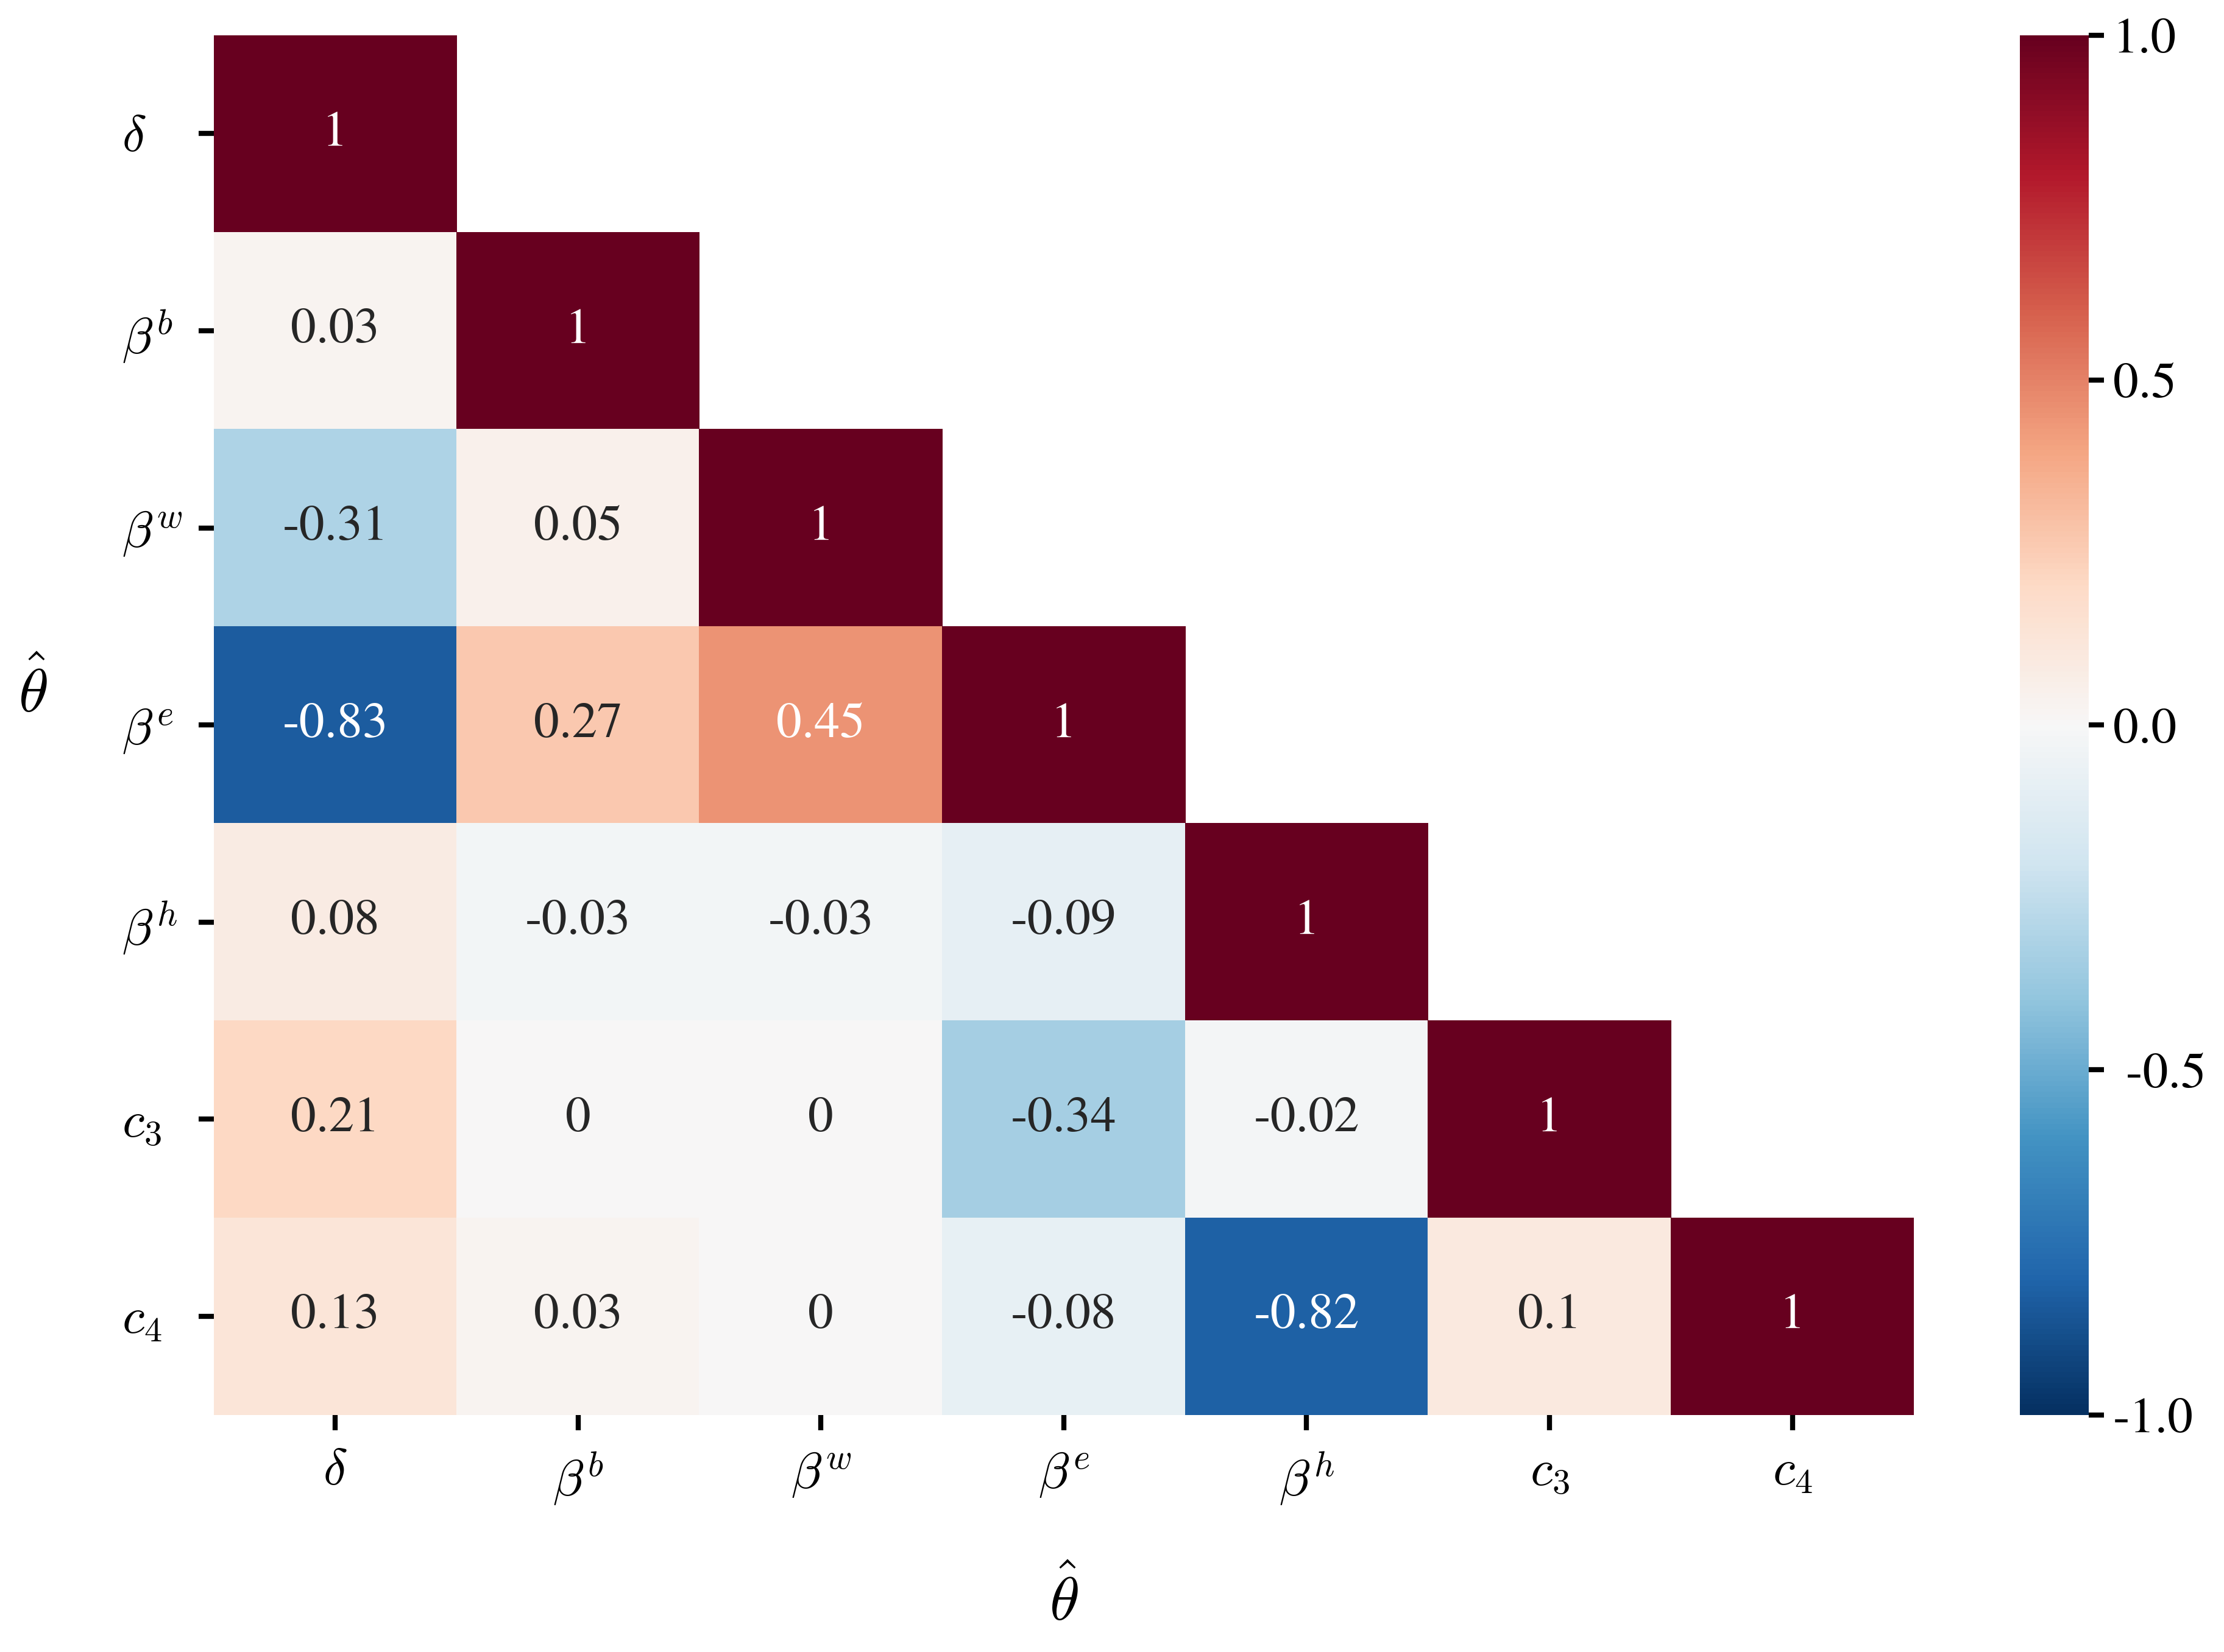
\includegraphics[scale=0.45]{../../../figures/heatmap_corr_chol}
	\label{fig:corr}
\end{figure}
\noindent
The intuition behind these results can be obtained from the following insight: Negative correlations imply similar effects, and positive correlations imply opposing effects on the likelihood of observed endogenous variables $\pmb{\mathcal{D}}$. For instance, consider an individual that decides for a long occupation in the education sector in the first years and then continues to work in the white-collar sector for the rest of his life. The likelihood to observe this individual increases when $\delta$ rises because all individuals get more patient, and therefore, ceteris paribus, they invest more in education. However, the same likelihood also increases if the educational utility constant $\beta^e$ rises. Hence, because they can compensate each other, the likelihood around the optimal parameter $\pmb{\hat{\theta}}$ decreases less for changes of both parameters in opposing directions than for changes in the same direction. Therefore, parameters $\delta$ and $\beta^e$ are negatively correlated in terms of the score function in (\ref{eq:scores}) around $\pmb{\hat{\theta}}$. It follows from (\ref{eq:est-cov}) that their standard errors are negatively correlated.

The above example provides intuition for $\text{corr}(\hat{\delta},\hat{\beta^e})=-0.83$ An analogous reasoning for the same example can explain $\text{corr}(\hat{\delta},\hat{\beta^w})=-0.31$. Yet, this correlation is smaller because $U_{w,t}$ has less covariates than $U_{e,t}$. $\text{corr}(\hat{c_3},\hat{\beta^e})=-0.34$ and $\text{corr}(\hat{c_4},\hat{\beta^h})=-0.82$ can be explained by a similar argument: Individuals decide for occupation in education or home sector if the respective utilities are high. This can be achieved by high constant terms or by high positive shocks. The latter can only happen to some individuals if the Cholesky factors are large because these factors are components of the respective shock variance. Shocks $\pmb{\varepsilon_{a,t}}$ are known to the agents prior to their decision $a_t$. Negative shocks have a smaller impact on choosing occupation $e$ or $h$ because individuals tend to decide against these alternatives anyway. Thus, $c_3$ and $\beta^e$, and $c_4$ and $\beta^h$ can impact the likelihood in the same direction. Therefore, their standard errors are negatively correlated. Moreover, the latter relationship is stronger because $U_{h,t}$ has a lower level and less covariates.


\subsection{Quantity of Interest}

The QoI is the effect of a 500 USD subsidy on annual tuition costs for higher education on the average years of education. Formally, $\beta_{he}^{e,pol} = \beta_{he}^e - 500$, where $\beta_{he}^{e,pol}$ represents the subsidised tuition costs. In KW94, the effect is an increase of 1.44 years.\footnote{See table 4, p. 668 in \cite{Keane.1994}.} The same figure computed with \citetalias{Respy-Stenzel.2019} is 1.5.\\
\newline
Figure \ref{fig:paths} depicts a comparison between the shares of occupations in the different sectors for a sample of 1000 individuals over their relevant lifetime between two different scenarios. The left graph shows the occupation paths under baseline parametrization $\hat{\theta}$ and the right graph the paths for the same model with subsidised tuition costs.

The red, blue, white, and green lines mark the shares of individuals occupied in the education, blue-collar, white-collar, and home sector, respectively. Both graphs show the typical life-cycle behaviour. Many agents tend to invest in their education early and continue in the white-collar sector as this sector rewards education. Another large group works in the blue-collar sector, and some of them switch to the white-collar sector, as well. This switch from white to blue-collar is caused by an accumulated blue-collar experience that is also rewarded in the white-collar sector and by positive shocks. The home sector is relatively irrelevant because the participation therein is comparably low for all ages.
\begin{figure}[H]
	\caption{Comparison of occupation paths between scenarios}
	\centering
	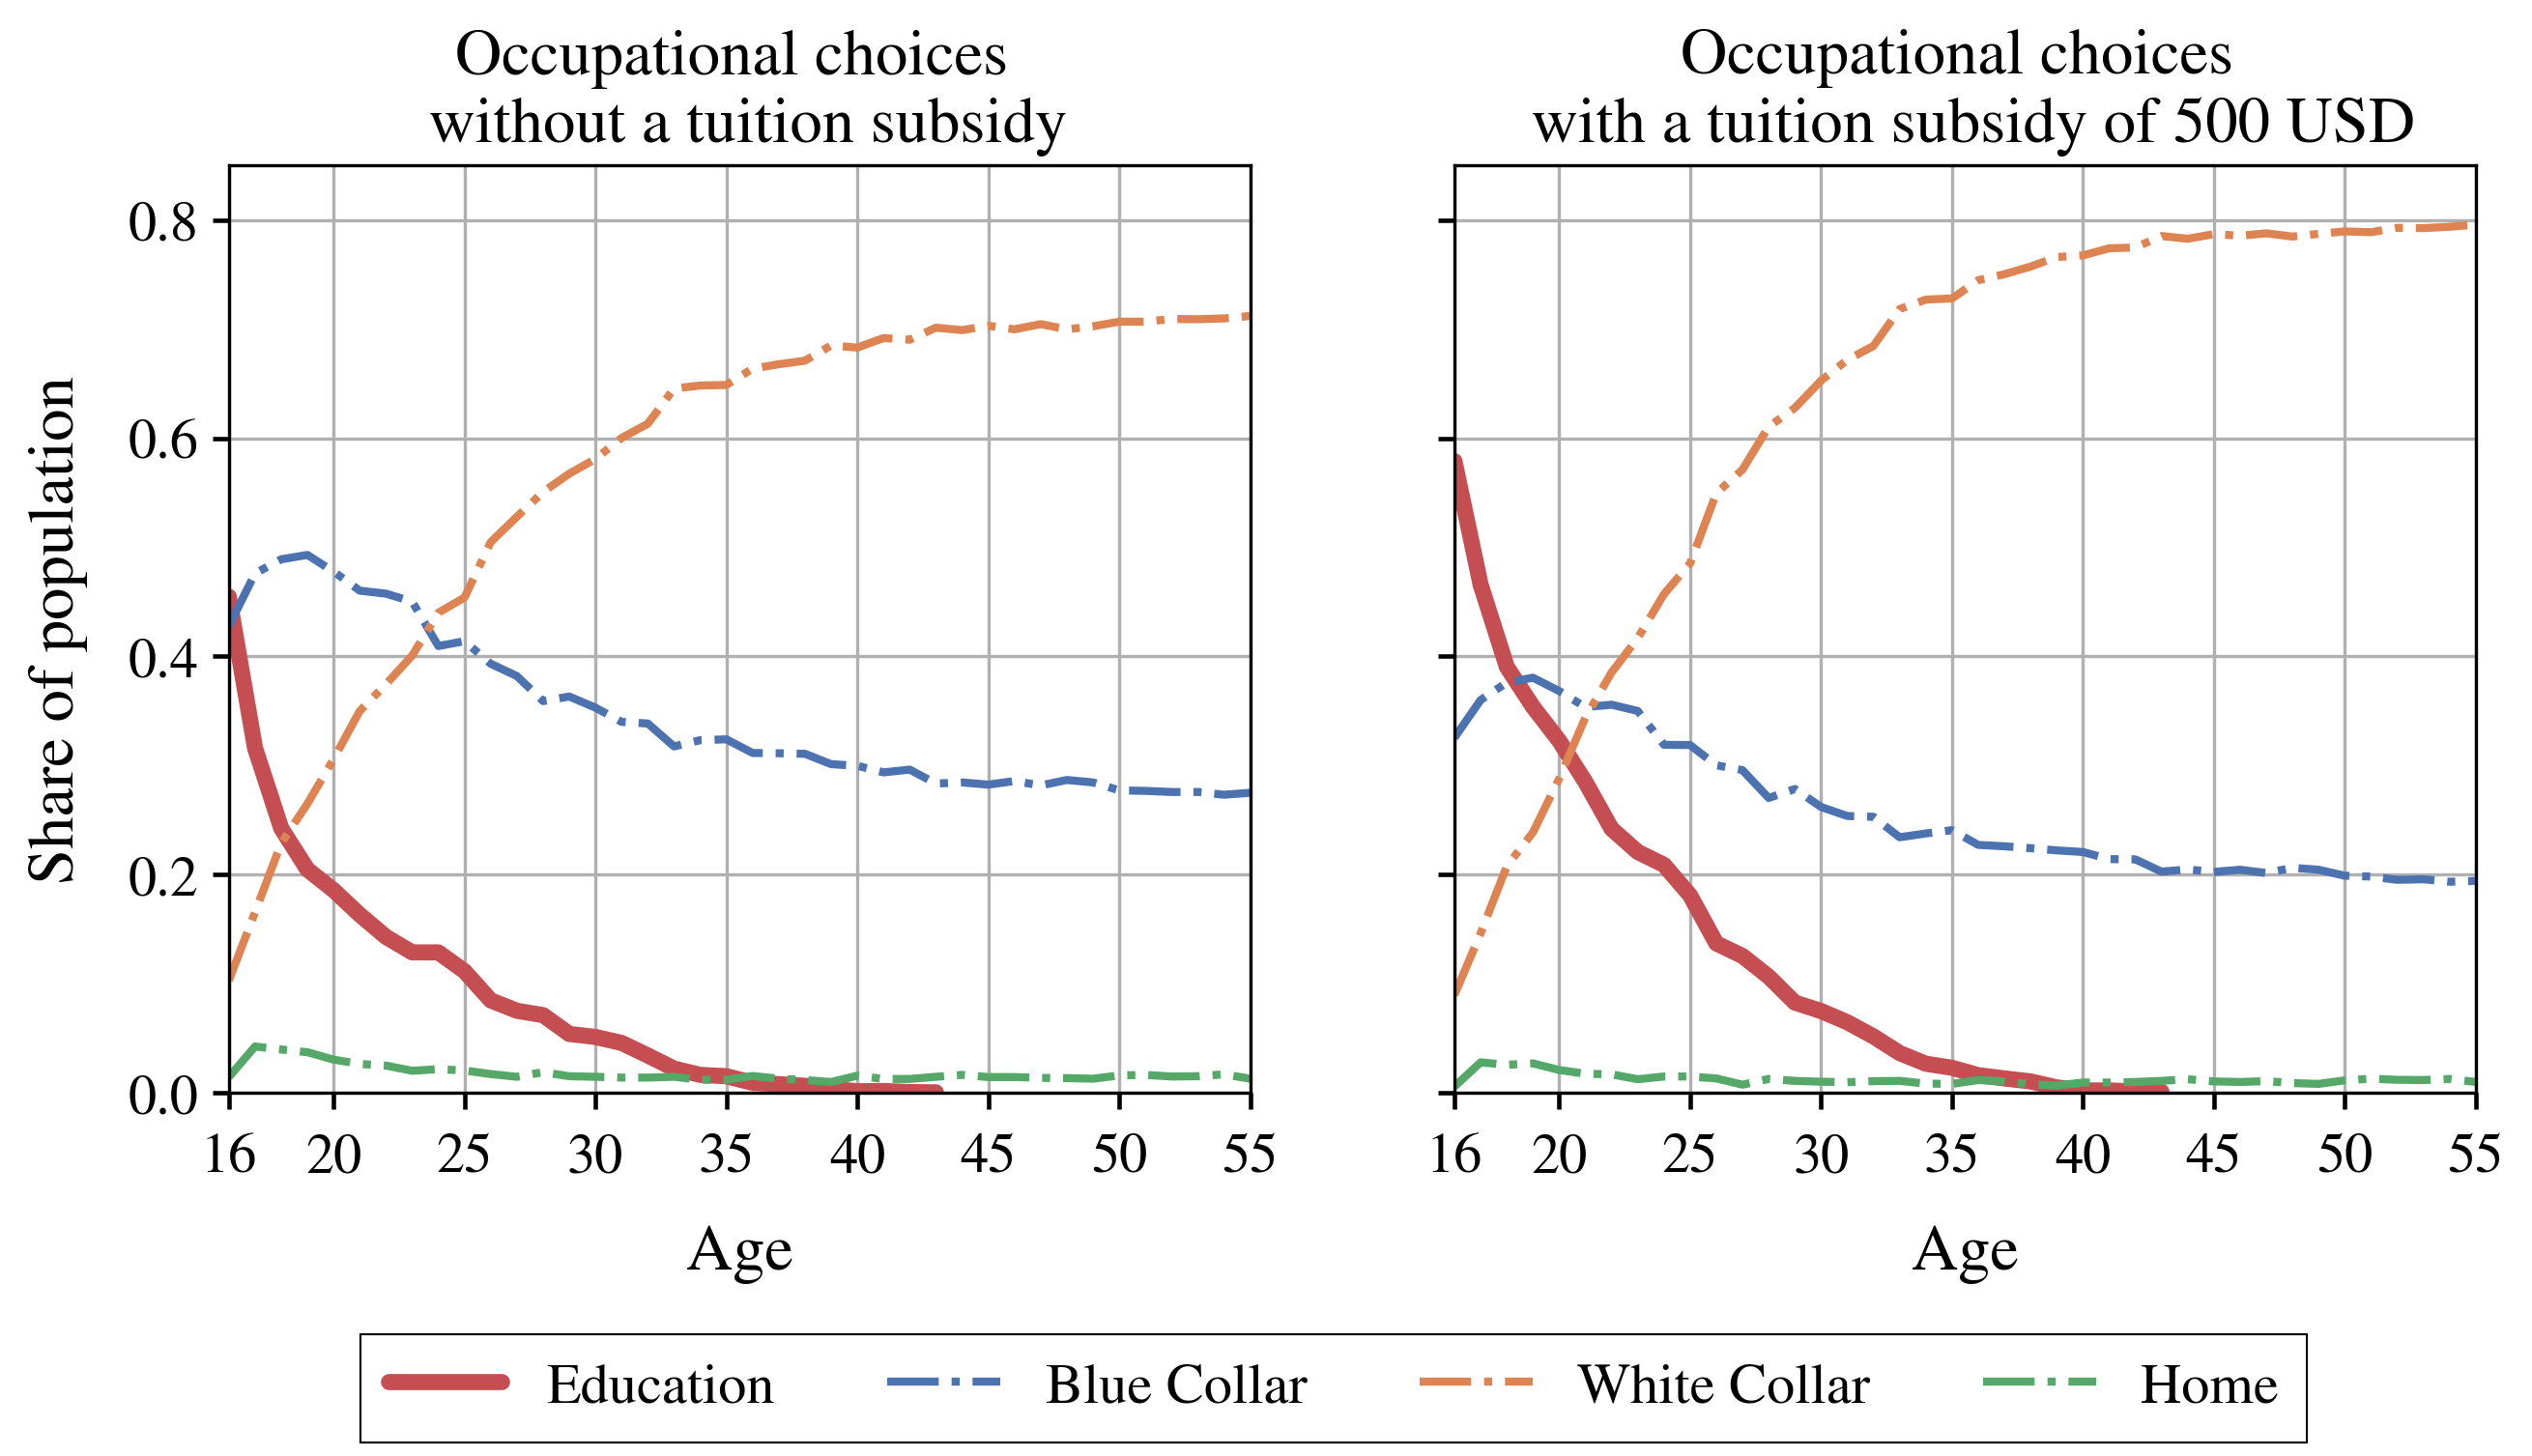
\includegraphics[scale=0.75]{../../../figures/occ_paths}
	\label{fig:paths}
\end{figure}
\noindent
The QoI is the sum of the differences between the education shares at each age in the right and in the left graph as depicted by the red lines.\footnote{If the red lines would depict continuous functions instead of discrete points in time, the QoI would be the difference between the integrals of the education shares as a function of time in the policy and the base scenario.} This is because the vertical axis can also be interpreted as the share of one year that the average agent is occupied in the education sector. Comparing both graphs, we can see that the tuition subsidy incentivises younger individuals to stay in the education sector for a longer time and older individuals to work in the white-collar sector. The latter observation is a consequence of the first because the white-collar sector rewards education.\\
\newline
The QoI, the impact of a 500 USD tuition subsidy for higher education on average schooling years, is chosen because it is relevant to society in many areas, for example, education, inequality, and economic growth. The discussion section expands on this point. The QoI's relevance allows me to illustrate the importance of UQ in economics in the context of political decisions.\\
\newline
The next section shows the results of the first part of the UQ, the uncertainty propagation.

% increase spacing between table columns
\setlength{\tabcolsep}{18pt} %from 6
\begin{table}[H] 
	\centering
	\begin{threeparttable}
		\caption[Model Parametrization]{Estimates for the distribution of input parameters}
		\label{tab:params}
		\renewcommand{\arraystretch}{1.2}%
		\begin{tabular}{cS[table-format=3.2]S[table-format=3.2]S[table-format=3.2]}
			\toprule
			{Parameter}     & {Mean}   & {Standard error (SE)} & {SE in KW94} \\ \midrule
			\textit{General} \\
			$\delta$ & 0.95   & 0.00084 & \textit{-}    \\    \midrule
			\textit{Blue-collar}\\    
			$\beta^b$ & 9.21   & .013            & 0.014      \\
			$\beta_e^b$ & 0.038  &    0.0011        & 0.0015       \\
			$\beta^b_b$ & 0.033  & 0.00044            & 0.00079       \\
			$\beta^b_{bb}$ & -0.0005 & 0.000013           & 0.000019       \\
			$\beta^b_w$ & 0.0    & 0.00067             & 0.0024      \\
			$\beta^b_{ww}$ & 0.0    & 0.000029           & 0.000096       \\ \midrule
			\textit{White-collar}\\
			$\beta^w$ & 8.48   & 0.0076             & 0.0123      \\
			$\beta^w_e$ & 0.07   & 0.00047          & 0.00096       \\
			$\beta^w_w$ & 0.067  & 0.00055            & 0.00090      \\
			$\beta^w_{ww}$ & -0.001  & 0.000017           & 0.000070     \\
			$\beta^w_b$ & 0.022  & 0.00033           & 0.0010      \\
			$\beta^w_{bb}$ & -0.0005 & 0.000021         & 0.000030      \\ \midrule
			\textit{Education} \\
			$\beta^e$     & 0.0    & 330                & 459       \\
			$\beta_{he}^e$     & 0.0    & 155               & 410       \\
			$\beta_{re}^e$     & -4000   & 202                & 660       \\ \midrule
			\textit{Home} \\
			$\beta^h$    & 17750  & 390                & 1442      \\ \midrule
			\multicolumn{4}{l}{\textit{Lower Triangular Cholesky Matrix}} \\
			$c_{1}$      & 0.2    & 0.0015             & 0.0056      \\
			$c_{2}$      & 0.25    & 0.0013             & 0.0046     \\
			$c_{3}$      & 1500   & 108             & 350      \\
			$c_{4}$      & 1500    & 173              & 786      \\
			$c_{1,2}$     & 0.0    & 0.0064              & 0.023     \\
			$c_{1,3}$      & 0.0   & 143               & 0.412      \\
			$c_{2,3}$      & 0.0    & 116             &  0.379     \\
			$c_{1,4}$      & 0.0    & 232             &   0.911    \\
			$c_{2,4}$      & 0.0    & 130            & 0.624      \\
			$c_{3,4}$      & 0.0   & 177                & 0.870       \\ \bottomrule
		\end{tabular}
	\end{threeparttable}
\end{table}

\newpage
\bibliography{../../../bibliography/literature}

\end{document}